% Fonte editável de fig/selecao_doador_primario_pt.pdf (Figura da seleção de
% doador primário dissimilar, Cap. 4, Seção 4.2.1). Esquemática: os pontos e as
% quantidades são ilustrativos e não vêm de nenhuma execução. O painel (b)
% segue IVF_V2.m:100-140: candidatos = metade da população de menor F; o
% doador secundário é excluído dos próprios candidatos; distâncias euclidianas
% sobre objetivos sem normalização; retêm-se os K = min(3, n_c) mais
% distantes; dois são sorteados e vence o de menor F. Os eixos têm a mesma
% escala, de modo que os três mais distantes no desenho são os três mais
% distantes em objetivos. No painel (b), o candidato em (0,68; 0,2403) é
% dominado por (0,55; 0,2067), logo tem F maior que o do candidato extremo
% (0,97; 0,0121), não dominado: por isso o extremo vence o torneio.
%
% Regenerar, a partir de thesis/masters/ (a primeira compilação baixa o TikZ;
% o build da dissertação só inclui o PDF e continua offline):
%   tectonic -o fig fig/src/selecao_doador_primario_pt.tex
\documentclass[border=2pt]{standalone}
\usepackage{fontspec}
\setmainfont{texgyreheros}[
  Extension = .otf,
  UprightFont = *-regular,
  BoldFont = *-bold,
]
\usepackage{tikz}
\usetikzlibrary{shapes.geometric,arrows.meta}

% Espaço de objetivos (f1, f2); fronteira f2 = 0,8 (1 - sqrt(f1)).
% Candidatos a doador primário (metade da população de menor F):
\def\candidatos{0.03/0.6614, 0.22/0.5148, 0.33/0.3404, 0.55/0.2067, 0.68/0.2403, 0.82/0.0756, 0.97/0.0121}
% Doador secundário (pertence à metade de menor F e é excluído dos próprios candidatos):
\def\sx{0.12}\def\sy{0.5229}
% Demais soluções da população:
\def\outras{0.07/0.8883, 0.30/0.6618, 0.45/0.4733, 0.60/0.5103, 0.86/0.2781, 0.20/0.9222, 0.42/0.7515}

\tikzset{
  outra/.style={circle, draw=black!50, fill=white, line width=0.6pt, inner sep=0pt, minimum size=4.4pt},
  candidato/.style={circle, draw=black!75, fill=black!35, line width=0.5pt, inner sep=0pt, minimum size=4.8pt},
  secundario/.style={regular polygon, regular polygon sides=3, draw=black, fill=black, inner sep=0pt, minimum size=8pt},
  primario/.style={star, star points=5, star point ratio=2.3, draw=black, fill=black, inner sep=0pt, minimum size=10.5pt},
  maisdistante/.style={circle, draw=black, line width=1.1pt, inner sep=0pt, minimum size=12pt},
  sorteado/.style={rectangle, draw=black, dash pattern=on 1.4pt off 1pt, line width=0.7pt, inner sep=0pt, minimum size=17pt},
  distancia/.style={black!60, line width=0.5pt, dash pattern=on 2pt off 1.5pt},
  recombina/.style={black, line width=0.7pt},
  titulo/.style={anchor=south west, font=\bfseries, inner sep=0pt},
}

\newcommand{\eixos}{%
  \draw[black!30, line width=0.6pt] plot[domain=0.01:1, samples=60, smooth] (\x, {0.8*(1 - sqrt(\x))});
  \draw[-{Latex[length=2mm]}, line width=0.6pt] (0,0) -- (1.10,0) node[below, inner sep=2pt] {$f_1$};
  \draw[-{Latex[length=2mm]}, line width=0.6pt] (0,0) -- (0,1.0) node[left, inner sep=2pt] {$f_2$};
}

\begin{document}
\fontsize{9}{11}\selectfont
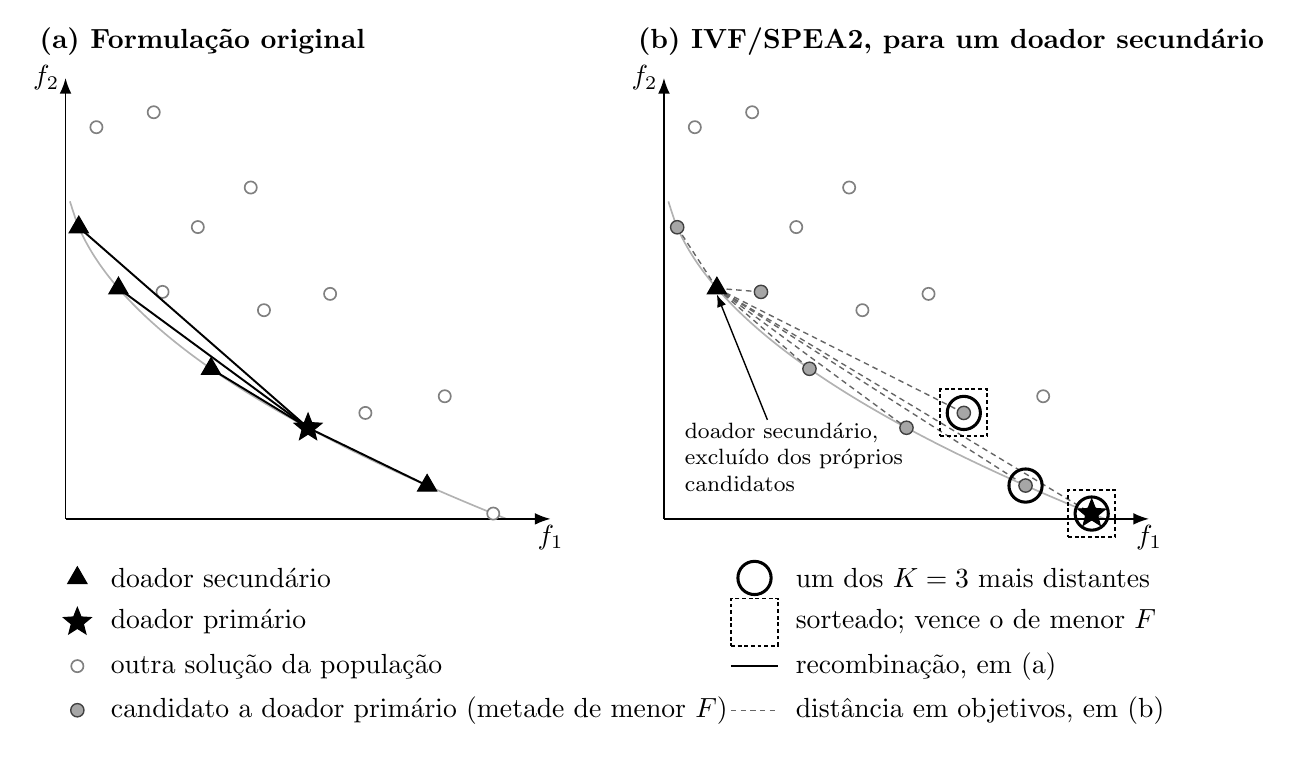
\begin{tikzpicture}[x=5.6cm, y=5.6cm]

  % ---------------- (a) formulação original ----------------
  \begin{scope}
    \eixos
    \node[titulo] at (-0.06,1.05) {(a) Formulação original};
    \foreach \x/\y in \outras { \node[outra] at (\x,\y) {}; }
    \foreach \x/\y in {0.22/0.5148, 0.68/0.2403, 0.97/0.0121} { \node[outra] at (\x,\y) {}; }
    % doador primário: o melhor indivíduo coletado, comum a todos
    \coordinate (P) at (0.55,0.2067);
    \foreach \x/\y in {0.03/0.6614, \sx/\sy, 0.33/0.3404, 0.82/0.0756} {
      \draw[recombina] (\x,\y) -- (P);
      \node[secundario] at (\x,\y) {};
    }
    \node[primario] at (P) {};
  \end{scope}

  % ---------------- (b) IVF/SPEA2 ----------------
  \begin{scope}[xshift=7.6cm]
    \eixos
    \node[titulo] at (-0.06,1.05) {(b) IVF/SPEA2, para um doador secundário};
    \foreach \x/\y in \candidatos { \draw[distancia] (\sx,\sy) -- (\x,\y); }
    \foreach \x/\y in \outras { \node[outra] at (\x,\y) {}; }
    \foreach \x/\y in \candidatos { \node[candidato] at (\x,\y) {}; }
    % os K = 3 mais distantes do doador secundário
    \foreach \x/\y in {0.68/0.2403, 0.82/0.0756, 0.97/0.0121} { \node[maisdistante] at (\x,\y) {}; }
    % dois sorteados entre os K
    \foreach \x/\y in {0.68/0.2403, 0.97/0.0121} { \node[sorteado] at (\x,\y) {}; }
    % vence o de menor F entre os dois sorteados
    \node[primario] at (0.97,0.0121) {};
    % doador secundário, excluído dos próprios candidatos
    \node[secundario] (S) at (\sx,\sy) {};
    \node[anchor=west, font=\footnotesize, align=left, inner sep=1pt] (rot) at (0.04,0.14)
      {doador secundário,\\excluído dos próprios\\candidatos};
    \draw[-{Latex[length=1.6mm]}, line width=0.5pt] (rot.north) ++(-0.06,0) -- (S.south);
  \end{scope}

  % ---------------- legenda ----------------
  \begin{scope}[x=1cm, y=1cm, shift={(0,-0.75)}]
    \def\lin{0.56}
    \node[secundario] at (0.15,0) {};         \node[anchor=west] at (0.45,0) {doador secundário};
    \node[primario] at (0.15,-\lin) {};       \node[anchor=west] at (0.45,-\lin) {doador primário};
    \node[outra] at (0.15,-2*\lin) {};        \node[anchor=west] at (0.45,-2*\lin) {outra solução da população};
    \node[candidato] at (0.15,-3*\lin) {};    \node[anchor=west] at (0.45,-3*\lin) {candidato a doador primário (metade de menor $F$)};
    \node[maisdistante] at (8.75,0) {};       \node[anchor=west] at (9.15,0) {um dos $K = 3$ mais distantes};
    \node[sorteado] at (8.75,-\lin) {};       \node[anchor=west] at (9.15,-\lin) {sorteado; vence o de menor $F$};
    \draw[recombina] (8.45,-2*\lin) -- (9.05,-2*\lin); \node[anchor=west] at (9.15,-2*\lin) {recombinação, em (a)};
    \draw[distancia] (8.45,-3*\lin) -- (9.05,-3*\lin); \node[anchor=west] at (9.15,-3*\lin) {distância em objetivos, em (b)};
  \end{scope}
\end{tikzpicture}
\end{document}
